\documentclass[11pt, a4paper]{article}

\usepackage[a4paper, margin=2.5cm]{geometry}
\usepackage[utf8]{inputenc}
\usepackage[T1]{fontenc}
% Magyar nyelv: a babel saját hungarian nyelvi beállítása (babel-hu.ini).
% A [magyar] opció helyett ez kell, mert a telepített magyar.ldf újabb a babel csomagnál,
% és a kettő együtt nem fordul le. Ez is magyar elválasztást, „Tartalomjegyzék”-et és „ábra” feliratot ad.
\usepackage{babel}
\babelprovide[import, main]{hungarian}
\usepackage{lmodern}
\usepackage{enumitem}
\setlist[itemize]{label=-}
\usepackage{booktabs}
\usepackage{graphicx} % Hozzáadva a nagyméretű UML ábrák szélességének auto-skálázásához
\usepackage{tikz} % Az állapotgép-ábrához
\usetikzlibrary{shapes.multipart, positioning, arrows.meta} % Az UML-ábrához
\usepackage[colorlinks=true, linkcolor=black, urlcolor=blue]{hyperref}
% A hosszú \texttt neveket nem lehet elválasztani; inkább kicsit nagyobb legyen a szóköz, mint hogy kilógjanak a margóra
\setlength{\emergencystretch}{3em}

% Magyar tipográfia: a fejezetszám után pont áll („1. A feladat”), az ábrafelirat „1. ábra” alakú
\makeatletter
\renewcommand{\@seccntformat}[1]{\csname the#1\endcsname.\quad}
\renewcommand{\fnum@figure}{\thefigure.~\figurename}
\makeatother

\usepackage{fancyhdr}
\pagestyle{fancy}
\fancyhf{}
\lhead{\textbf{PAC-MAN}}
\rhead{Tari Balázs}
\cfoot{\thepage}
\renewcommand{\headrulewidth}{0.4pt}

\begin{document}

% --- Címlap ---
\begin{titlepage}
    \centering
    \vspace*{4cm}
    {\Huge \textbf{PAC-MAN} \par}
    \vspace{1.5cm}
    {\LARGE A programozás alapjai 3. \par}
    \vspace{0.5cm}
    {\Large Feladatspecifikáció \par}
    
    \vspace{4.5cm}
    
    {\Large \textbf{Tari Balázs} \par}
    \vspace{0.3cm}
    {\Large E3K6W5 \par}
    
    \vfill
    
    {\large 2026. október 16. \par}
    \vspace{0.2cm}
\end{titlepage}

% --- Tartalomjegyzék ---
\tableofcontents
\newpage

% --- 1. A feladat ---
\section{A feladat}
A Pac-Man egy kétdimenziós asztali arcade játék. A játékos a sárga figurát irányítja egy labirintusban; a feladata, hogy összegyűjtse az összes pöttyöt, és közben elkerülje a pályán mozgó szellemeket. Ha Pac-Man felveszi a labirintusban található 4 power pellet egyikét, 6 másodpercig megeheti a szellemeket, és ezzel további pontokat szerez.

A program grafikus felülete a Java Swing keretrendszerre épül, a játékállapot tartós tárolását fájlkezelés biztosítja, a kód minőségét pedig automatizált JUnit egységtesztek ellenőrzik.

% --- 2. Használati esetek ---
\section{Használati esetek (use case-ek)}
\begin{enumerate}
    \item \textbf{A játék indítása és irányítása:} A felhasználó a menüből indít új játékot: megnyílik egy fájlválasztó ablak a \texttt{maps} mappában, és kiválasztja, melyik pályán szeretne játszani (alapértelmezetten a beépített \texttt{level1.txt} van kijelölve). Pac-Mant a labirintusban a WASD billentyűkkel lehet irányítani.
    \item \textbf{Pöttyök gyűjtése és győzelem:} Amikor Pac-Man áthalad a pöttyökön, azok eltűnnek, és nő a pontszám. Ha az összes pötty és power pellet elfogyott, a játékos a következő szintre lép: ugyanaz a labirintus jön újra, minden pöttyel, a pontszám és a megmaradt életek pedig megmaradnak. Magasabb szinteken rövidebb az ijedt (Frightened) állapot, ezért nehezebb a játék. Az állapotsor mindig mutatja az aktuális szintet.
    \item \textbf{Ütközés a szellemekkel:} Ha a karakter összeütközik egy szellemmel, életet veszít. Ha az életek száma nullára csökken, a játék véget ér (Game Over). Új játék indításakor a játékos mindig az első szinten kezd.
    \item \textbf{A legjobb eredmények mentése:} Amikor az utolsó élet is elfogy, a rendszer fájlba menti az elért pontszámot. A főmenü \textit{Leaderboard} képernyője az összes rögzített eredményt mutatja, a legjobbtól a leggyengébbig.
    \item \textbf{A játékállás mentése:} Játék közben az állapotsor \textit{SAVE \& QUIT} gombja vagy az F5 billentyű menti a játékot: a játékos egy mentési párbeszédablakban adja meg a fájl nevét, ezután a játék visszatér a főmenübe. Tetszőleges számú játék menthető. A főmenü \textit{Load previous game} gombja fájlválasztót nyit, és a kiválasztott mentés pontosan ott folytatódik, ahol abbamaradt.
    \item \textbf{Pályaszerkesztő mód:} Az alapjátékon felül a felhasználó a \textit{Create map} gombbal saját pályákat rajzolhat, ezeket a \texttt{maps} mappába mentheti, és később játszhat rajtuk, ha a \textit{Start new game} után kiválasztja őket. Minden pálya akkora, mint a beépített pálya ($19 \times 21$ mező), és a középen lévő szellemház (Ghost House) rögzített: a felhasználó körülötte rajzolja meg a falakat, a pöttyöket, a power pelleteket és Pac-Man kezdőmezőjét.
\end{enumerate}

% --- 3. A megoldás vázlatos ismertetése ---
\section{A megoldás vázlatos ismertetése}
\begin{enumerate}
    \item \textbf{Alkalmazott technológiák:} Java SE, Swing (JFrame, JPanel, CardLayout a képernyők közötti váltáshoz, JFileChooser a fájlok kiválasztásához, Graphics az alacsony szintű rajzoláshoz, \texttt{javax.swing.Timer} a másodpercenként 60 tickes játékciklushoz), valamint JUnit 5 az automatizált teszteléshez.
    \item \textbf{Fájlformátumok:} egyszerű CSV fájl a ranglistához, a pálya szöveges „rajza” (mezőnként egy karakter) a pályákhoz, és Java bináris szerializáció a mentett játékállásokhoz (mentésenként egy \texttt{.dat} fájl a \texttt{saves} mappában). Lásd: \ref{sec:io}.~fejezet.
\end{enumerate}

\clearpage

% --- 4. Részletes architektúra és osztályszerkezet ---
\section{Részletes architektúra és osztályszerkezet}

\textbf{A játék magja (modell)}
\begin{itemize}
    \item \textbf{GameEngine:} A játék központi vezérlője. Ő adja a játékciklus egy tickjét (\texttt{update()}), amelyet a \texttt{GamePanel} Swing \texttt{Timer}-e hív meg (lásd: \ref{sec:game_loop}.~fejezet), frissíti a játék állapotát (pozíciók, ütközések), és kezeli a pontszámot, a megmaradt életeket és az aktuális szintet (\texttt{currentLevel}). Az aktív játékállás mentése és betöltése is az ő feladata (a \texttt{java.io.Serializable} segítségével). A szint növekedésével a szellemek ijedt állapotának időtartama fokozatosan csökken, így nő a nehézség; Pac-Man és a szellemek normál sebessége minden szinten ugyanaz. Új játék a \texttt{LevelManager} által felépített \texttt{LevelData} objektumból indul, mindig 0 ponttal, 3 élettel és az 1. szinten. A motor egyetlen, közös \texttt{java.util.Random} példányt használ a szellemek véletlen döntéseihez; egy második konstruktor egy megadott \texttt{Random}-ot fogad, így a tesztek rögzített seeddel (kezdőértékkel) minden futáskor ugyanazokat a döntéseket kapják.

    \textbf{Szintlépés:} Létrehozáskor a motor eltesz egy érintetlen másolatot a labirintusról (\texttt{originalMap}, a \texttt{Labyrinth.copy()} készíti). Ha már nem maradt pötty vagy power pellet (a \texttt{Labyrinth.hasDotsLeft()} \texttt{false}-t ad), a lépés végén a \texttt{nextLevel()} fut le:
    \begin{itemize}
        \item a \texttt{currentLevel} eggyel nő;
        \item minden mező visszamásolódik az \texttt{originalMap}-ből, így minden pötty és power pellet visszakerül;
        \item Pac-Man és az összes szellem a \texttt{resetToStart()} hívással visszaáll a kezdőmezőjére;
        \item az ijedtség-időzítő és a szellemevési sorozat nullázódik;
        \item a pontszám és a megmaradt életek megmaradnak.
    \end{itemize}
    A mezők ugyanabba a \texttt{Labyrinth} objektumba másolódnak vissza, ahelyett hogy a motor lecserélné azt. Így a \texttt{map} adattag maradhat \texttt{final}, a modell sosem olvas fájlt, és senkinél (például egy pufferelt \texttt{MoveCommand}-nál) sem marad referencia egy régi labirintusra. Minden szinten ugyanaz a labirintus jön.

    \textbf{Mentés és betöltés:} A \texttt{saveGameState(file)} metódus fájlba írja ezt a motort, a \texttt{loadGameState(file)} metódus pedig \textbf{statikus gyártómetódus} (static factory): egy vadonatúj, a fájlból beolvasott \texttt{GameEngine}-t ad vissza, ahelyett hogy egy meglévőt töltene fel, mert a legtöbb adattag (\texttt{map}, \texttt{pacman}, \texttt{ghosts}, \texttt{random}, \ldots) \texttt{final}, és a létrehozás után nem kaphat új értéket. Ugyanez az elv, mint amikor a \texttt{LevelManager} \texttt{loadFromCSV} metódusa új \texttt{LevelData}-t ad vissza. Lásd: \ref{sec:io}.~fejezet.
    \item \textbf{Labyrinth:} A pályát reprezentáló osztály. Minden mező típusát (fal, pötty, power pellet, üres) egy kétdimenziós tömbben tárolja, \texttt{grid[row][column]} indexeléssel. Egy mező járható, ha nem fal, és a tömbön kívüli pozíciók falnak számítanak, így semmi sem hagyhatja el a pályát. Kereszteződés az a járható mező, amelynek legalább három járható szomszédja van. A \texttt{hasDotsLeft()} megmondja, maradt-e még \texttt{DOT} vagy \texttt{POWERPELLET}; az első találatnál megáll. A \texttt{copy()} mély másolatot ad a labirintusról a szint pillanatképéhez: minden sort új tömbbe másol (\texttt{Arrays.copyOf}), mert egy kétdimenziós tömbön a \texttt{clone()} csak a sorokra mutató referenciákat másolná, és egy pötty megevése a pillanatképet is megváltoztatná. A \texttt{Labyrinth} nem olvas fájlt; a pályákat a \texttt{LevelManager} tölti be.
    \item \textbf{GameObject} (absztrakt ősosztály): A mozgó szereplők közös tulajdonságait fogja össze (X és Y koordináta, sebesség, irány). A pozíciók \textbf{mezőkoordináták}: az \texttt{x} a labirintus oszlopa, az \texttt{y} a sora, a \texttt{speed} pedig azt adja meg, hány teljes mezőt tesz meg egy lépés. Az aktuális mezőn kívül minden objektum még kettőt megjegyez:
    \begin{itemize}
        \item a \textbf{kezdőmezőjét} (\texttt{startX}, \texttt{startY}, \texttt{final}), ahová a \texttt{resetToStart()} visszahelyezi, álló helyzetben, miután Pac-Man életet veszített;
        \item az \textbf{előző mezőjét} (\texttt{prevX}, \texttt{prevY}), amelyet a \texttt{rememberPosition()} minden lépés elején elment, akkor is, ha az objektum nem mozdul. A nézet ennek segítségével csúsztatja simán a szereplőt két mező között, az ütközésvizsgálat pedig ebből ismeri fel, ha két szereplő áthaladt egymáson.
    \end{itemize}
    \begin{itemize}
        \item \textbf{PacMan} (leszármazott osztály): A játékos karakterének állapotát tárolja, és kezeli a bemenetet: a legutóbbi billentyűlenyomás \texttt{Command}-ként pufferelődik, és a következő lépésben fut le. Felüldefiniálja a \texttt{resetToStart()}-ot: az ősosztály változatának meghívása után a pufferelt parancsot is eldobja, így a halál előtt lenyomott billentyű nem indítja el rögtön újra Pac-Mant. A \texttt{currentCommand} adattag \texttt{transient}: kimarad a mentésből, és a betöltött játék pufferelt billentyű nélkül indul (lásd: \ref{sec:io}.~fejezet).
        \item \textbf{Ghost} (leszármazott osztály): A szellemek állapotát tárolja és a mozgásukat irányítja. A \texttt{possibleDirections()} felsorolja az aktuális mezőről járható irányokat, visszafordulás nélkül, kivéve, ha a szellem zsákutcában van. Két metódus választ közülük: a \texttt{chooseDirection()} véletlenszerűen, a \texttt{chooseDirectionTowards(target)} pedig azt az irányt, amelynek a következő mezője a legközelebb van egy célmezőhöz (lásd: \ref{sec:game_loop}.~fejezet). A \texttt{chooseChaseDirection()} a szellem stratégiaobjektumától kéri el a célmezőt (lásd: \ref{sec:design_patterns}.~fejezet), és arrafelé lép; ha egy személyiséghez még nincs stratégia, a szellem véletlenszerűen választ. Folyosóban vagy kanyarban csak egy irány marad, így valódi döntés csak kereszteződésben történik. Az állapotváltásokat események váltják ki, mindegyiknek saját metódusa van: \texttt{frighten()}, \texttt{calmDown()}, \texttt{eaten()} és \texttt{respawn()}. A szellem is felüldefiniálja a \texttt{resetToStart()}-ot: az ősosztály változata után visszaállítja az állapotát \texttt{CHASE}-re, így Pac-Man életvesztése után egyetlen szellem sem marad ijedt vagy halott.
    \end{itemize}
    \item \textbf{LevelData:} Egyszerű adattároló egy pályafájl tartalmához: a \texttt{Labyrinth}, Pac-Man a kezdőmezőjén és a szellemek a kezdőmezőjükön. A \texttt{LevelManager} hozza létre, a \texttt{GameEngine} pedig a részeiből épül fel.
\end{itemize}

\vspace{0.3cm}
\textbf{Felhasználói felület és kezelőosztályok}
\begin{itemize}
    \item \textbf{MainFrame (JFrame):} Az alkalmazás főablaka. Egy \texttt{CardLayout} vált a képernyők között: a menü, az aktív játék, a ranglista és a szerkesztő. A \texttt{switchScreen(name)} megjelenít egy képernyőt; a ranglistára váltás előtt először meghívja a \texttt{LeaderboardPanel} \texttt{refresh()} metódusát, így a legutóbbi megtekintés óta hozzáadott eredmény is mindig megjelenik, és ezt egyik gombnak sem kell külön megjegyeznie. A \texttt{startGame(engine)} felépíti a \texttt{GamePanel}-t egy új vagy egy betöltött játékhoz, és megjeleníti; a \texttt{quitGame()} visszavisz a menübe. Egyszerre csak egy játékképernyő létezik (\texttt{currentGame}): amikor a játékos kilép egy játékból, a program a panelt leállítja és eltávolítja, nem csak elrejti, mert egy rejtett panel \texttt{Timer}-e tovább futna a háttérben. A szerkesztőt ugyanígy kezeli: az \texttt{openEditor()} minden alkalommal vadonatúj \texttt{MapEditor}-t épít (így az mindig üres pályával indul), a \texttt{closeEditor()} pedig eltávolítja. Az ablak mérete (\texttt{pack()}) mindig a megjelenített képernyőhöz igazodik.
    \item \textbf{MainMenu (JPanel):} A kezdőképernyő: a sárga \textit{PAC-MAN} cím és négy középre igazított gomb fekete háttéren: \textit{Start new game} (\texttt{startBtn}), \textit{Load previous game} (\texttt{loadGameBtn}), \textit{Leaderboard} (\texttt{leaderboardBtn}) és \textit{Create map} (\texttt{editorBtn}). A \textit{Start new game} fájlválasztót nyit a \texttt{maps} mappában, a \texttt{level1.txt} kijelölésével; a kiválasztott pályát a \texttt{LevelManager.loadFromCSV} olvassa be, és új játék indul rajta (0 pont, 3 élet, 1. szint); hiányzó vagy hibás pálya esetén csak hibaüzenet jelenik meg. A fájl betöltése a menü feladata, így a \texttt{GamePanel} mindig kész \texttt{GameEngine}-t kap. A \textit{Load previous game} fájlválasztót nyit a \texttt{saves} mappában, a kiválasztott fájlt a \texttt{GameEngine.loadGameState} tölti be, majd a \texttt{MainFrame} megjeleníti a játékot; ha a fájl nem tölthető be, hibaüzenet jelenik meg, és a menü marad.
    \item \textbf{GamePanel (JPanel):} Az aktív játék képernyője, amely összeköti a modellt és a nézetet. A WASD billentyűlenyomásokat \texttt{MoveCommand} objektumokká alakítja, a \texttt{GameEngine}-től megkapja a játék állapotát, és a \texttt{paintComponent} metódusában kirajzolja a labirintust és a szereplőket. A szereplők az előző és az aktuális mezőjük között jelennek meg, a lépésen belüli előrehaladás szerint, így a mozgás folyamatosnak látszik, pedig a modell egész mezőkkel dolgozik. A szellem színe a személyiségét mutatja (\texttt{TRACKER} piros, \texttt{AMBUSHER} rózsaszín, \texttt{WANDERER} narancssárga, \texttt{CHAOTIC} cián, hogy a sötétkék falak mellett is jól látsszon). Az állapot felülírja a személyiséget: az ijedt szellem fehér, a \texttt{DEAD} szellem pedig csak egy kis szürke pont (a szeme).
    \begin{itemize}
        \item \textbf{Állapotsor (HUD):} a pontszám, a megmaradt életek, az aktuális szint, a \texttt{GAME OVER} felirat, ha már nincs élet, és a jobb szélén egy \textit{SAVE \& QUIT} gomb. A gomb valódi \texttt{JButton} gyerekkomponens (a panel abszolút pozicionálással helyezi el), és nem kaphatja meg a billentyűzetfókuszt, különben egy kattintás után a panel nem kapná meg többé a WASD billentyűket.
        \item \textbf{Mentés és kilépés:} a gomb és az F5 billentyű ugyanazt a metódust hívja. Ez szünetelteti a \texttt{Timer}-t (egy modális párbeszédablak is feldolgozza a Swing eseményeket, így a játék tovább futna mögötte), egy mentési párbeszédablakban bekéri a fájlt, ment, majd visszalép a menübe. Ha a játékos megszakítja, vagy az írás nem sikerül, a játék egyszerűen folytatódik, így semmi sem vész el. Game Over után azonnal, mentés nélkül lép vissza a menübe: egy befejezett játékban már semmi sem történhet, és egy ilyen mentés betöltése másodszor is beírná ugyanazt a pontszámot a ranglistába. A pontszám ekkorra már rögzítve van, mert a játékot lezáró \texttt{Timer}-tick beírta, a gombkattintás pedig ugyanazon a szálon (az EDT-n) csak e tick után fut le.
        \item \textbf{Legjobb eredmény:} a játék végén a panel pontosan egyszer írja be a pontszámot a \texttt{highscores.csv}-be (egy jelző őrzi, mert az \texttt{isGameOver()} minden további tickben igaz marad). A játékos neve a \texttt{System.getProperty("user.name")} hívásból származik. A fájlírás a felhasználói felület dolga; a modell sosem nyúl fájlhoz.
        \item A panel nem ismeri a \texttt{MainFrame}-et: a keret \texttt{Runnable} visszahívásként (\texttt{onQuit}) adja át neki a „vissza a menübe” műveletet, a panel pedig csak jelzi, hogy a játékos kilépett.
    \end{itemize}
    \item \textbf{LeaderboardPanel (JPanel):} A \texttt{highscores.csv} csak olvasható nézete: helyezés, játékosnév, pontszám és dátum, játékonként egy sor, a legjobb elöl, fix szélességű betűtípussal, hogy az oszlopok egymás alá kerüljenek, és egy \textit{Back to menu} gombbal. A fájlt sosem írja. A \texttt{refresh()} minden megjelenítéskor újraolvassa a fájlt; a ranglista csak két játék között változik, ezért nincs szükség időzítőre. Ha még nincs fájl, a „No scores yet” szöveget mutatja.
    \item \textbf{HighscoreEntry (record):} A ranglista egy sora (\texttt{playerName}, \texttt{score}, valamint \texttt{date} \texttt{LocalDate}-ként). Csak adatot szállít a \texttt{LevelManager} és a \texttt{LeaderboardPanel} között, ezért a felhasználói felület és az I/O csomagjába tartozik, nem a játékmodellbe.
    \item \textbf{MapEditor (JPanel):} Az egyéni pályák rajzolására szolgáló képernyő: középen egy kattintható rács, jobbra az eszköztár, felül a \textit{BACK} és a \textit{SAVE MAP} gomb.
    \begin{itemize}
        \item \textbf{Rögzített méret és szellemház:} a rács mindig $19 \times 21$ mezős (\texttt{MAP\_WIDTH}, \texttt{MAP\_HEIGHT}), akkora, mint a \texttt{level1.txt}, és üresen (feketén) indul. A szellemház a \texttt{level1.txt}-ből van átmásolva, és egy kis sablonként tárolódik, a pályafájl jeleivel (\texttt{GHOST\_HOUSE}): a 7--11. oszlop és a 8--10. sor (0-tól számozva) $5 \times 3$-as blokkja, benne az \texttt{AMBUSHER}, a \texttt{WANDERER} és a \texttt{CHAOTIC} szellemmel, valamint a \texttt{TRACKER} mezője a felső nyílás fölött. Ezek a mezők zárolva vannak (\texttt{isLocked}), sötétszürke padlón jelennek meg, és a négy szellem mindig itt kezd; a felhasználó nem helyezhet el szellemet. Ez eltér az eredeti tervtől, amelyben a szellemek kezdőmezője is elhelyezhető volt.
        \item \textbf{Eszközök:} négy kapcsológomb egy \texttt{ButtonGroup}-ban, így mindig pontosan egy van kiválasztva: \textit{WALL}, \textit{DOT}, \textit{POWER PELLET}, \textit{PAC-MAN START}. Minden gombon egy előnézet látható, amelyet ugyanaz a kód rajzol, mint a rácsot.
        \item \textbf{Rajzolás:} a bal egérgomb a kiválasztott eszközzel rajzol, kattintásra, vagy lenyomva tartva minden mezőre, amelyen az egér áthalad (\texttt{mousePressed} és \texttt{mouseDragged}); a jobb egérgomb üres padlóvá törli a mezőt. A program a \texttt{SwingUtilities.isLeftMouseButton} és \texttt{isRightMouseButton} metódust használja, mert ezek húzás közben is működnek. A rácson kívüli pozíciókat és a zárolt mezőket figyelmen kívül hagyja.
        \item \textbf{Pac-Man kezdőmezője} egyetlen adattag (\texttt{pacmanStart}), nem egy jel a rácsban, így sosem lehet belőle kettő: újbóli lerakáskor áthelyeződik. Pac-Man csak üres padlón állhat, ezért ha bármit a mezőjére rajzolunk, eltűnik.
        \item \textbf{SAVE MAP:} először ellenőrzi a pályát: Pac-Man kezdőmezőjének lerakva kell lennie, és legalább egy pöttynek kell lennie (a pötty nélküli pálya azonnal „teljesítve” lenne, és a motor minden lépésben szintet lépne). Azt nem ellenőrzi, hogy minden pötty elérhető-e. Ezután mentési párbeszédablak nyílik a \texttt{maps} mappában; a kiterjesztés nélküli névhez hozzáadja a \texttt{.txt}-t, a \texttt{level1.txt} nem írható felül, egy másik meglévő pályát pedig csak megerősítés után ír felül. A pályát a \texttt{LevelManager.saveToCSV} írja ki, így pontosan abban a formátumban, amelyet a játék beolvas. Mentés után a szerkesztő nyitva marad.
        \item \textbf{BACK:} visszalép a menübe; ha a pályán mentetlen változás van (\texttt{unsaved}), előbb rákérdez. A \texttt{GamePanel}-hez hasonlóan a szerkesztő sem ismeri a \texttt{MainFrame}-et: a „vissza a menübe” műveletet \texttt{Runnable}-ként kapja meg (\texttt{onBack}).
    \end{itemize}
    \item \textbf{LevelManager (Factory):} Önálló, állapot nélküli osztály, amely egy pályafájlt \texttt{LevelData}-vá olvas be (labirintus, Pac-Man és a szellemek), és egy \texttt{LevelData}-t ugyanebben a formátumban ír vissza pályafájlba (lásd: \ref{sec:custom_maps}.~fejezet). Ő kezeli a ranglistát is (\texttt{loadHighscores}, \texttt{appendHighscore}), és itt vannak a rögzített fájl- és mappanevek (\texttt{HIGHSCORES\_FILE}, \texttt{MAPS\_DIR}, \texttt{DEFAULT\_MAP\_NAME}, \texttt{SAVES\_DIR}, \texttt{DEFAULT\_SAVE\_NAME}).
\end{itemize}



\begin{figure}[h!]
    \centering
    \resizebox{\textwidth}{!}{ % Ráhúzza a diagramot a maximális lapszélességre
    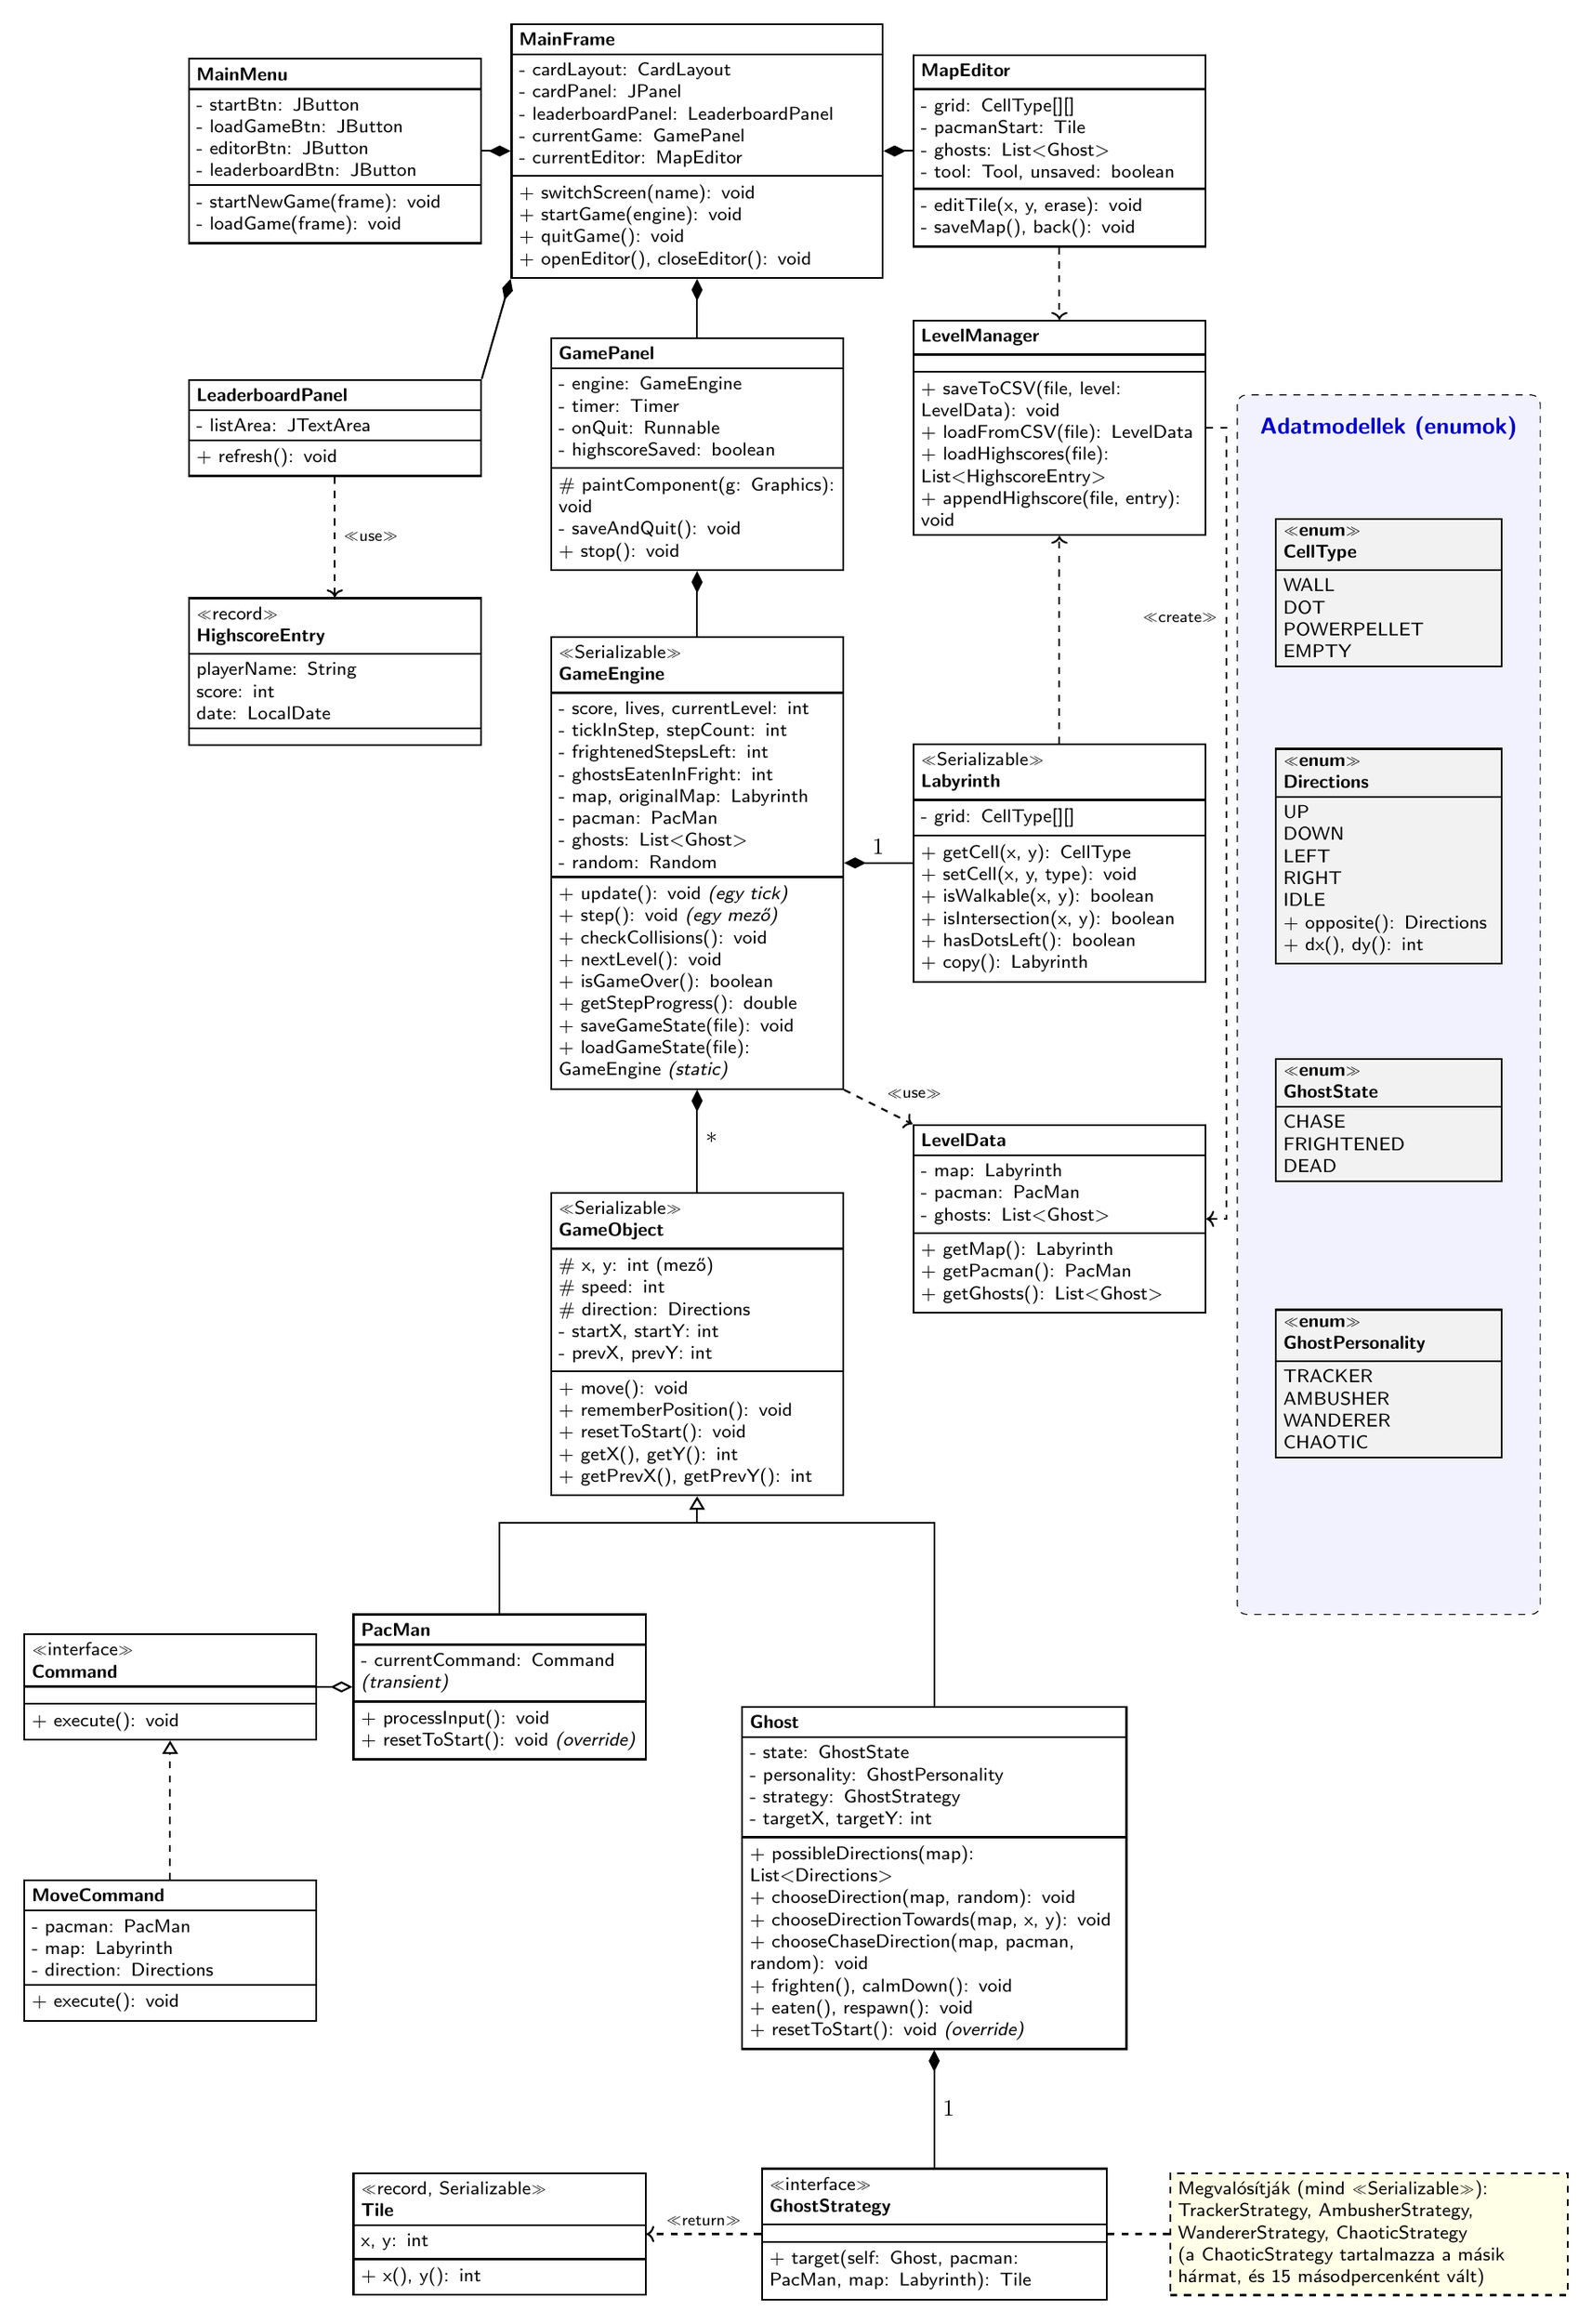
\begin{tikzpicture}[
        umlclass/.style={
            draw, thick,
            rectangle split,
            rectangle split parts=3,
            font=\sffamily\footnotesize, % Olvashatóbb, nagyobb betűméret
            align=left,
            text width=4.2cm,
            fill=white
        },
        umlenum/.style={
            draw, thick,
            rectangle split,
            rectangle split parts=2,
            font=\sffamily\footnotesize,
            align=left,
            text width=3.2cm,
            fill=gray!10
        }
    ]
        
        % === FELHASZNÁLÓI FELÜLET ÉS KEZELŐOSZTÁLYOK ===
        \node[umlclass, text width=5.4cm] (MainFrame) at (0, 8.2) {
            \textbf{MainFrame}
            \nodepart{two}
            - cardLayout: CardLayout \\
            - cardPanel: JPanel \\
            - leaderboardPanel: LeaderboardPanel \\
            - currentGame: GamePanel \\
            - currentEditor: MapEditor
            \nodepart{three}
            + switchScreen(name): void \\
            + startGame(engine): void \\
            + quitGame(): void \\
            + openEditor(), closeEditor(): void
        };

        \node[umlclass] (MainMenu) at (-5.5, 8.2) {
            \textbf{MainMenu}
            \nodepart{two}
            - startBtn: JButton \\
            - loadGameBtn: JButton \\
            - editorBtn: JButton \\
            - leaderboardBtn: JButton
            \nodepart{three}
            - startNewGame(frame): void \\
            - loadGame(frame): void
        };

        \node[umlclass] (LeaderboardPanel) at (-5.5, 4.0) {
            \textbf{LeaderboardPanel}
            \nodepart{two}
            - listArea: JTextArea
            \nodepart{three}
            + refresh(): void
        };

        \node[umlclass] (HighscoreEntry) at (-5.5, 0.3) {
            \guillemotleft record\guillemotright \\
            \textbf{HighscoreEntry}
            \nodepart{two}
            playerName: String \\
            score: int \\
            date: LocalDate
            \nodepart{three}
        };

        \node[umlclass] (MapEditor) at (5.5, 8.2) {
            \textbf{MapEditor}
            \nodepart{two}
            - grid: CellType[][] \\
            - pacmanStart: Tile \\
            - ghosts: List$<$Ghost$>$ \\
            - tool: Tool, unsaved: boolean
            \nodepart{three}
            - editTile(x, y, erase): void \\
            - saveMap(), back(): void
        };

        \node[umlclass] (LevelManager) at (5.5, 4.0) {
            \textbf{LevelManager}
            \nodepart{two}
            % Nincs belső állapot (Utility/Factory)
            \nodepart{three}
            + saveToCSV(file, level: LevelData): void \\
            + loadFromCSV(file): LevelData \\
            + loadHighscores(file): List$<$HighscoreEntry$>$ \\
            + appendHighscore(file, entry): void
        };

        \node[umlclass] (GamePanel) at (0, 3.6) {
            \textbf{GamePanel}
            \nodepart{two}
            - engine: GameEngine \\
            - timer: Timer \\
            - onQuit: Runnable \\
            - highscoreSaved: boolean
            \nodepart{three}
            \# paintComponent(g: Graphics): void \\
            - saveAndQuit(): void \\
            + stop(): void
        };


        % === A JÁTÉK MAGJA (MODELL) ===
        \node[umlclass] (GameEngine) at (0, -2.6) {
            \guillemotleft Serializable\guillemotright \\
            \textbf{GameEngine}
            \nodepart{two}
            - score, lives, currentLevel: int \\
            - tickInStep, stepCount: int \\
            - frightenedStepsLeft: int \\
            - ghostsEatenInFright: int \\
            - map, originalMap: Labyrinth \\
            - pacman: PacMan \\
            - ghosts: List$<$Ghost$>$ \\
            - random: Random
            \nodepart{three}
            + update(): void \textit{(egy tick)} \\
            + step(): void \textit{(egy mező)} \\
            + checkCollisions(): void \\
            + nextLevel(): void \\
            + isGameOver(): boolean \\
            + getStepProgress(): double \\
            + saveGameState(file): void \\
            + loadGameState(file): GameEngine \textit{(static)}
        };

        \node[umlclass] (Labyrinth) at (5.5, -2.6) {
            \guillemotleft Serializable\guillemotright \\
            \textbf{Labyrinth}
            \nodepart{two}
            - grid: CellType[][]
            \nodepart{three}
            + getCell(x, y): CellType \\
            + setCell(x, y, type): void \\
            + isWalkable(x, y): boolean \\
            + isIntersection(x, y): boolean \\
            + hasDotsLeft(): boolean \\
            + copy(): Labyrinth
        };

        \node[umlclass] (GameObject) at (0, -9.9) {
            \guillemotleft Serializable\guillemotright \\
            \textbf{\textit{GameObject}}
            \nodepart{two}
            \# x, y: int (mező) \\
            \# speed: int \\
            \# direction: Directions \\
            - startX, startY: int \\
            - prevX, prevY: int
            \nodepart{three}
            + move(): void \\
            + rememberPosition(): void \\
            + resetToStart(): void \\
            + getX(), getY(): int \\
            + getPrevX(), getPrevY(): int
        };

        \node[umlclass] (PacMan) at (-3, -15.1) {
            \textbf{PacMan}
            \nodepart{two}
            - currentCommand: Command \textit{(transient)}
            \nodepart{three}
            + processInput(): void \\
            + resetToStart(): void \textit{(override)}
        };
        
        \node[umlclass] (Command) at (-8, -15.1) {
            \guillemotleft interface\guillemotright \\
            \textbf{Command}
            \nodepart{two}
            \nodepart{three}
            + execute(): void
        };

        \node[umlclass, text width=5.6cm] (Ghost) at (3.6, -18.0) {
            \textbf{Ghost}
            \nodepart{two}
            - state: GhostState \\
            - personality: GhostPersonality \\
            - strategy: GhostStrategy \\
            - targetX, targetY: int
            \nodepart{three}
            + possibleDirections(map): List$<$Directions$>$ \\
            + chooseDirection(map, random): void \\
            + chooseDirectionTowards(map, x, y): void \\
            + chooseChaseDirection(map, pacman, random): void \\
            + frighten(), calmDown(): void \\
            + eaten(), respawn(): void \\
            + resetToStart(): void \textit{(override)}
        };

        \node[umlclass] (MoveCommand) at (-8, -19.1) {
            \textbf{MoveCommand}
            \nodepart{two}
            - pacman: PacMan \\
            - map: Labyrinth \\
            - direction: Directions
            \nodepart{three}
            + execute(): void
        };

        \node[umlclass] (LevelData) at (5.5, -8.0) {
            \textbf{LevelData}
            \nodepart{two}
            - map: Labyrinth \\
            - pacman: PacMan \\
            - ghosts: List$<$Ghost$>$
            \nodepart{three}
            + getMap(): Labyrinth \\
            + getPacman(): PacMan \\
            + getGhosts(): List$<$Ghost$>$
        };

        \node[umlclass, text width=5.0cm] (GhostStrategy) at (3.6, -23.4) {
            \guillemotleft interface\guillemotright \\
            \textbf{GhostStrategy}
            \nodepart{two}
            \nodepart{three}
            + target(self: Ghost, pacman: PacMan, map: Labyrinth): Tile
        };

        \node[umlclass] (Tile) at (-3, -23.4) {
            \guillemotleft record, Serializable\guillemotright \\
            \textbf{Tile}
            \nodepart{two}
            x, y: int
            \nodepart{three}
            + x(), y(): int
        };

        \node[draw, dashed, thick, font=\sffamily\footnotesize, align=left, text width=5.8cm, fill=yellow!10] (StrategyNote) at (10.2, -23.4) {
            Megvalósítják (mind \guillemotleft Serializable\guillemotright): \\
            TrackerStrategy, AmbusherStrategy, \\
            WandererStrategy, ChaoticStrategy \\
            (a ChaoticStrategy tartalmazza a másik \\
            hármat, és 15 másodpercenként vált)
        };

        % === ADATMODELLEK (ENUMOK) SZUPERÁLT BLOKK ===
        % Dedikált, halvány hátterű keret az enumoknak
       \draw[dashed, fill=blue!5, rounded corners] (8.2, 4.5) rectangle (12.8, -14.0);
        \node[font=\sffamily\bfseries, text=blue!80!black] at (10.5, 4.0) {Adatmodellek (enumok)};

        \node[umlenum] (CellType) at (10.5, 1.5) {
            \textbf{\guillemotleft enum\guillemotright \\ CellType}
            \nodepart{two}
            WALL \\ DOT \\ POWERPELLET \\ EMPTY
        };

        \node[umlenum] (Directions) at (10.5, -2.5) {
            \textbf{\guillemotleft enum\guillemotright \\ Directions}
            \nodepart{two}
            UP \\ DOWN \\ LEFT \\ RIGHT \\ IDLE \\
            + opposite(): Directions \\
            + dx(), dy(): int
        };

        \node[umlenum] (GhostState) at (10.5, -6.5) {
            \textbf{\guillemotleft enum\guillemotright \\ GhostState}
            \nodepart{two}
            CHASE \\ FRIGHTENED \\ DEAD
        };

        \node[umlenum] (GhostPersonality) at (10.5, -10.5) {
            \textbf{\guillemotleft enum\guillemotright \\ GhostPersonality}
            \nodepart{two}
            TRACKER \\ AMBUSHER \\ WANDERER \\ CHAOTIC
        };

        % === KAPCSOLATOK ===
        % UI dependenciák és kompozíciók
        \draw[{Diamond[fill=black, scale=1.2]}-, thick] (MainFrame.west) -- (MainMenu.east);
        \draw[{Diamond[fill=black, scale=1.2]}-, thick] (MainFrame.east) -- (MapEditor.west);
        \draw[{Diamond[fill=black, scale=1.2]}-, thick] (MainFrame.south) -- (GamePanel.north);
        \draw[{Diamond[fill=black, scale=1.2]}-, thick] (MainFrame.south west) -- (LeaderboardPanel.north east);
        \draw[dashed, ->, thick] (LeaderboardPanel.south) -- (HighscoreEntry.north) node[midway, right, font=\sffamily\scriptsize] {\guillemotleft use\guillemotright};
        
        \draw[dashed, ->, thick] (MapEditor.south) -- (LevelManager.north);
        \draw[dashed, ->, thick] (Labyrinth.north) -- (LevelManager.south);
        \draw[{Diamond[fill=black, scale=1.2]}-, thick] (GamePanel.south) -- (GameEngine.north);

        % Modell kapcsolatok
        \draw[{Diamond[fill=black, scale=1.2]}-, thick] (GameEngine.east) -- (Labyrinth.west) node[midway, above] {1};
        \draw[{Diamond[fill=black, scale=1.2]}-, thick] (GameEngine.south) -- (GameObject.north) node[midway, right] {*};

        % Öröklődés
        \draw[-{Triangle[open, fill=white, scale=1.2]}, thick] ([yshift=-0.4cm]GameObject.south) -- (GameObject.south);
        \draw[thick] (PacMan.north) |- ([yshift=-0.4cm]GameObject.south);
        \draw[thick] (Ghost.north) |- ([yshift=-0.4cm]GameObject.south);
        
        % Command minta: aggregáció
        \draw[{Diamond[fill=white, scale=1.2]}-, thick] (PacMan.west) -- (Command.east);
        % A MoveCommand megvalósítja a Command interfészt
        \draw[dashed, -{Triangle[open, fill=white, scale=1.2]}, thick] (MoveCommand.north) -- (Command.south);

        % LevelData: a LevelManager hozza létre, a GameEngine ebből épül fel
        \draw[dashed, ->, thick] (LevelManager.east) -- ++(0.3, 0) |- (LevelData.east) node[pos=0.12, left, font=\sffamily\scriptsize] {\guillemotleft create\guillemotright};
        \draw[dashed, ->, thick] (GameEngine.south east) -- (LevelData.north west) node[midway, above right, font=\sffamily\scriptsize] {\guillemotleft use\guillemotright};

        % Strategy minta: a szellem birtokolja a stratégiaobjektumát
        \draw[{Diamond[fill=black, scale=1.2]}-, thick] (Ghost.south) -- (GhostStrategy.north) node[midway, right] {1};
        \draw[dashed, thick] (GhostStrategy.east) -- (StrategyNote.west);
        \draw[dashed, ->, thick] (GhostStrategy.west) -- (Tile.east) node[midway, above, font=\sffamily\scriptsize] {\guillemotleft return\guillemotright};

    \end{tikzpicture}
    } % \resizebox vége
    \caption{A teljes játékarchitektúra UML osztálydiagramja}
    \label{fig:uml_complete_diagram}
\end{figure}

\clearpage

\section{Játékciklus, mozgás és ütközések}
\label{sec:game_loop}
A modell egész mezőkkel dolgozik, a képernyő viszont másodpercenként 60-szor rajzolódik újra. A kettőt a \textit{tick} (ütem) és a \textit{lépés} (step) szétválasztása tartja külön:
\begin{itemize}
    \item \textbf{Tick:} A \texttt{GamePanel} Swing \texttt{Timer}-e $1000 / \texttt{TICKS\_PER\_SECOND}$ ms-onként ($\approx$16 ms) jelez, meghívja a \texttt{GameEngine.update()}-et, majd a \texttt{repaint()}-et. Egy \texttt{update()} egy tick.
    \item \textbf{Lépés:} Az \texttt{update()} minden \texttt{TICKS\_PER\_STEP} (= 10) tickben meghívja a \texttt{step()}-et, amely minden szereplőt legfeljebb egy mezővel mozgat. Másodpercenként 60 tick mellett ez 6 mező másodpercenként. Minden játékszabály (bemenet, mozgás, ütközések, pontozás) a \texttt{step()}-ben fut, ezért az egységtesztek közvetlenül a \texttt{step()}-et hívják, és nem függenek az időzítéstől.
    \item \textbf{Folyamatos rajzolás (interpoláció):} A \texttt{getStepProgress()} megadja, hol tart az aktuális lépés, 0.0 és 1.0 között. A \texttt{GamePanel} minden szereplőt a $(\textit{előző} + (\textit{aktuális} - \textit{előző}) \cdot \textit{haladás}) \cdot \textit{TILE}$ pixelpozícióra rajzol. A pixelszámítás csak a nézetben él; a modell sosem foglalkozik pixelekkel. Mellékhatásként a kép legfeljebb egy lépéssel ($\approx$166 ms) lemarad a modell mögött.
    \item \textbf{Időtartamok:} Minden időtartamot (az ijedt állapot hosszát, a Chaotic szellem 15 másodperces váltását) a \texttt{TICKS\_PER\_SECOND} segítségével számol át a program másodpercből, így a tickgyakoriság megváltoztatásához elég egyetlen konstanst átírni.
\end{itemize}

\textbf{Egy lépés sorrendje:}
\begin{enumerate}
    \item Ha a játék véget ért, semmi sem történik.
    \item Ha fut az ijedtség-időzítő, eggyel csökken; amikor eléri a 0-t, minden szellem megkapja a \texttt{calmDown()} hívást. Ez még a mozgás előtt történik, így ebben a lépésben a szellemek már teljes sebességgel mozognak.
    \item Pac-Man végrehajtja a pufferelt parancsát, amely elfordítja, ha a kívánt irányban szabad a mező, majd lép egy mezőt, hacsak nem fal van előtte.
    \item Minden szellem az állapota szerint irányt választ, és lép:
    \begin{itemize}
        \item \texttt{DEAD}: a szellemházban lévő saját kezdőmezője felé (\texttt{chooseDirectionTowards});
        \item \texttt{FRIGHTENED}: véletlenszerűen, és csak minden \texttt{FRIGHTENED\_STEP\_INTERVAL} (= 2). lépésben, így feleakkora a sebessége; a kihagyott lépésekben is meghívja a \texttt{rememberPosition()}-t;
        \item egyébként: a stratégiája által megadott célmező felé (\texttt{chooseChaseDirection}).
    \end{itemize}
    A lépése után a \texttt{respawn()} visszaállítja \texttt{CHASE}-re azt a \texttt{DEAD} szellemet, amely éppen elérte a kezdőmezőjét. Fontos, hogy ez a lépés után fusson: a saját kezdőmezőjén megevett szellemnek előbb el kell hagynia azt, különben azonnal feltámadna.
    \item Az ütközésvizsgálat akkor fut le, amikor már mindenki lépett.
    \item Ha nem maradt pötty vagy power pellet, a \texttt{nextLevel()} elindítja a következő szintet. Ez az ütközésvizsgálat után jön, mert az eszi meg az utolsó pöttyöt, és az számolja el a pontját.
\end{enumerate}
Mozgás előtt minden szereplő elmenti az előző mezőjét a \texttt{rememberPosition()} hívással, akkor is, ha egy helyben áll. Különben a nézet újra lejátszaná az utolsó csúszást, az ütközésvizsgálat pedig régi mezőket hasonlítana össze.

\textbf{A szellemek mozgási szabályai:} A szellem sosem fordul vissza 180 fokban, kivéve zsákutcában, ahol a visszafordulás az egyetlen kiút, és egyszer, amikor ijedt állapotba kerül. Folyosóban vagy kanyarban csak egy irány marad, így a szellem valójában csak kereszteződésben dönt.

\textbf{Célmező-alapú útvonalválasztás (Target Tile Routing):} A szellem minden döntésnél azt az irányt választja a lehetséges irányok közül (\texttt{possibleDirections()}), amelynek a következő mezője a legközelebb van a célmezőhöz; ezt a \texttt{chooseDirectionTowards(target)} metódus végzi. Ez \textit{mohó} (greedy) választás: az adott pillanatban legjobbnak tűnő lépés, előretervezés nélkül, pontosan úgy, mint az eredeti játékban. Nem mindig a legrövidebb utat találja meg, ettől a szellemek kiszámíthatók, de nem tökéletesek. A távolság az egyenes vonalú távolság négyzete, $dx^2 + dy^2$; a négyzetgyökvonás elmarad, mert nem változtat azon, melyik távolság a kisebb, így a számítás egész számokkal történik. Egyenlőség esetén a listában előbb álló irány nyer (\texttt{UP}, \texttt{DOWN}, \texttt{LEFT}, \texttt{RIGHT}). A célmező lehet falon vagy a labirintuson kívül is; csak mérhetőnek kell lennie, elérhetőnek nem. A kiválasztott célmező a \texttt{targetX}, \texttt{targetY} adattagba kerül.

\textbf{Ütközések:}
\begin{itemize}
    \item \textbf{Pöttyök és power pelletek:} Ha Pac-Man egy \texttt{DOT} (10 pont) vagy egy \texttt{POWERPELLET} (50 pont) mezőn fejezi be a lépést, nő a pontszám, és a mező \texttt{EMPTY} lesz. A power pellet minden szellemen meghívja a \texttt{frighten()}-t, (újra)indítja az ijedtség-időzítőt, és nullázza a szellemevési sorozatot.
    \item \textbf{Az ijedtség időtartama:} A \texttt{frightenedDurationSteps()} az aktuális szintből olvassa ki az időtartamot, és lépésekre váltja át ($\textit{másodperc} \cdot \texttt{TICKS\_PER\_SECOND} / \texttt{TICKS\_PER\_STEP}$, előbb szorozva, hogy az egészosztás ne vágjon le törtrészt):

    \vspace{0.1cm}
    \begin{tabular}{@{}lll@{}}
        \toprule
        \textbf{Szint} & \textbf{Másodperc} & \textbf{Lépés} \\
        \midrule
        1--3 & 6 & 36 \\
        4--6 & 4 & 24 \\
        7--10 & 2 & 12 \\
        11+ & 1 & 6 \\
        \bottomrule
    \end{tabular}
    \vspace{0.1cm}

    Az időtartam sosem lesz 0: egy 0 lépéses ijedtség fehérré tenné és megfordítaná a szellemeket, a visszaszámlálás pedig örökre ijedten hagyhatná őket. Egy új power pellet a teljes időtartamot újraindítja.
    \item \textbf{Pac-Man és egy szellem} akkor találkozik, ha a lépés után ugyanazon a mezőn állnak, \textit{vagy} helyet cseréltek: Pac-Man ott áll, ahol korábban a szellem, \textit{és} a szellem ott áll, ahol korábban Pac-Man. A helycsere-feltétel mindkét fele kell; egyik önmagában akkor is igaz lenne, amikor Pac-Man egyszerűen követ egy szellemet. A vizsgálat pontos, mert minden szereplő lépésenként legfeljebb egy mezőt mozog.
    \item \textbf{Az ütközés jelentése a szellem állapotától függ,} és a program két menetben dönti el, így az eredmény nem függ a szellemek listabeli sorrendjétől:
    \begin{enumerate}
        \item minden ütköző \texttt{FRIGHTENED} szellemet megeszik (\texttt{eatGhost()}); nincs korai kilépés, így Pac-Man egy lépésben két szellemet is megehet;
        \item ezután bármely ütköző, nem \texttt{DEAD} szellem megöli Pac-Mant. Az első menetben megevett szellemek ekkorra már \texttt{DEAD} állapotúak, a \texttt{DEAD} szellemek (csak a szemük) pedig ártalmatlanok.
    \end{enumerate}
    \item \textbf{Szellem megevése:} A szellem \texttt{DEAD} állapotba kerül (\texttt{eaten()}). Egy ijedtségen belül a megevett szellemek 200, 400, 800 és 1600 pontot érnek: $200 \cdot 2^n$, ahol $n$ az utolsó power pellet óta már megevett szellemek száma, legfeljebb 3, így egy több szellemes egyéni pályán minden további szellem is 1600 pontot ér. Javában a $2^n$ \texttt{1 << n} alakban írható; a \texttt{\^{}} operátor bitenkénti XOR.
    \item \textbf{Életvesztés:} Halálos ütközéskor a \texttt{lives} eggyel csökken, az ijedtség-időzítő nullázódik, Pac-Man és \textit{az összes} szellem pedig a \texttt{resetToStart()} hívással visszakerül a kezdőmezőjére (minden szellem újra \texttt{CHASE}); a megevett pöttyök megevettek maradnak. Lépésenként legfeljebb egy élet veszhet el: a második menet az első találat után megáll.
    \item \textbf{Game Over:} Az \texttt{isGameOver()} az életekből számolódik (\texttt{lives <= 0}), nem egy külön jelzőben tárolódik, így a kettő sosem mondhat ellent egymásnak. Ha igaz, a \texttt{step()} azonnal visszatér, semmi sem mozdul többé, a \texttt{GamePanel} pedig egyszer beírja a pontszámot a ranglistába.
\end{itemize}

\clearpage

% --- 6. Tervezési minták ---
\section{Tervezési minták}
\label{sec:design_patterns}
Annak érdekében, hogy a kód megfeleljen az egyetemi elvárásoknak, és jól mutassa az objektumorientált elveket, a megvalósításnak kifejezetten a következő tervezési mintákat kell alkalmaznia:

\begin{itemize}
    \item \textbf{A szellemek mozgása (Strategy minta):} Minden személyiség célmező-számítása külön osztályban van (\texttt{TrackerStrategy}, \texttt{AmbusherStrategy}, \texttt{WandererStrategy}, \texttt{ChaoticStrategy}), és mindegyik ugyanazt a \texttt{GhostStrategy} interfészt valósítja meg, amelynek egyetlen metódusa van: \texttt{Tile target(Ghost self, PacMan pacman, Labyrinth map)}. A célmező \texttt{Tile}-ként tér vissza, ami egy kis, módosíthatatlan (immutable) \texttt{record} \texttt{x} és \texttt{y} adattaggal, mert egy metódus csak egy értéket adhat vissza (a \texttt{java.awt.Point} nem jöhet szóba, mert a modell nem függhet az AWT-től). A stratégia csak azt mondja meg, \textit{hová} menjen a szellem; azt, hogy \textit{hogyan} kerüljön közelebb, a \texttt{chooseDirectionTowards} dönti el. Azt, hogy egy szellem melyik stratégiát kapja, a \texttt{GhostPersonality} enum határozza meg (a konstruktorban a \texttt{Ghost.strategyFor()}), a \texttt{Ghost} pedig adattagként tárolja (öröklés helyett kompozíció).

    \textbf{A személyiségek célmezői:}
    \begin{itemize}
        \item \textbf{TRACKER} (piros): pontosan Pac-Man saját mezője; bárhová követi. \textit{(megvalósítva: \texttt{TrackerStrategy})}
        \item \textbf{AMBUSHER} (rózsaszín): 4 mezővel Pac-Man előtt, abban az irányban, amerre néz, a \texttt{Directions.dx()} és \texttt{dy()} segítségével számolva (lépésenként $-1$, $0$ vagy $+1$). Ha Pac-Man egy helyben áll, a célmező a saját mezője. \textit{(megvalósítva: \texttt{AmbusherStrategy})}
        \item \textbf{WANDERER} (narancssárga): Pac-Man mezője, de a saját, szellemházbeli kezdőmezője, ha 8 mezőnél közelebb kerül hozzá (a távolság négyzete kisebb, mint $8^2 = 64$; a pontosan 8 mezőre lévő szellem még üldöz). Amint újra legalább 8 mezőre van, ismét Pac-Man felé fordul, így folyamatosan váltogat az üldözés és a visszavonulás között. \textit{(megvalósítva: \texttt{WandererStrategy})}
        \item \textbf{CHAOTIC} (cián): tartalmazza a másik három stratégiát, és 15 másodpercenként ($15 \cdot \texttt{TICKS\_PER\_SECOND} / \texttt{TICKS\_PER\_STEP} = 90$ lépés) véletlenszerűen átvált valamelyikre (akár ugyanarra is). A visszaszámlálás a \texttt{target()} hívásaiban mér, üldözés közben lépésenként egyben, így szünetel, amíg a szellem ijedt vagy halott: a 15 másodperc 15 másodpercnyi üldözést jelent. Minden kaotikus szellemnek saját példánya van, a \texttt{Random} pedig átadható a konstruktornak, így a tesztek minden futáskor ugyanazokat a váltásokat kapják. \textit{(megvalósítva: \texttt{ChaoticStrategy})}
    \end{itemize}
    Mind a négy személyiségnek megvan a stratégiája; egy stratégia nélküli szellem továbbra is véletlenszerűen választana. Ennek a tervnek a Chaotic szellem az oka: egy objektum futás közben nem változtathatja meg az osztályát, egy szellem viszont lecserélheti a stratégiaobjektumát. A \texttt{ChaoticStrategy} saját állapotot tart nyilván (a 15 másodperces időzítőt és az éppen aktív stratégiát), és a másik három között vált. Mivel minden szellem a stratégiájával együtt mentődik, a stratégiaosztályoknak meg kell valósítaniuk a \texttt{java.io.Serializable} interfészt.
    \item \textbf{A szellemek viselkedése (véges állapotgép, FSM):} A szellemek aktuális üzemmódját a \texttt{GhostState} enum kezeli (\texttt{CHASE}, \texttt{FRIGHTENED}, \texttt{DEAD}). Az állapotok közötti átmeneteket szigorúan a játék eseményei irányítják, ahogy az állapotgép-ábra (\ref{fig:ghost_fsm}.~ábra) mutatja. Minden eseménynek saját metódusa van a \texttt{Ghost} osztályban, egyetlen, bármilyen állapotot elfogadó publikus setter helyett, így a kód élről élre követi az ábrát:

    \vspace{0.1cm}
    \begin{tabular}{@{}lll@{}}
        \toprule
        \textbf{Esemény (él)} & \textbf{Metódus} & \textbf{Melyik állapotból} \\
        \midrule
        Power pellet & \texttt{frighten()} & minden állapotból, kivéve \texttt{DEAD} \\
        Lejár az ijedtség & \texttt{calmDown()} & csak \texttt{FRIGHTENED} \\
        Pac-Man megeszi & \texttt{eaten()} & csak \texttt{FRIGHTENED} \\
        Hazaér & \texttt{respawn()} & \texttt{DEAD}, a kezdőmezőjén \\
        \bottomrule
    \end{tabular}
    \vspace{0.1cm}

    Minden metódus maga ellenőrzi a saját feltételét, és ha az nem teljesül, nem csinál semmit, így rossz állapotban meghívni ártalmatlan (például a \texttt{calmDown()} békén hagyja a \texttt{DEAD} szellemet). A motor csak jelzi az eseményt; a szellem dönti el, hogy vonatkozik-e rá. Pac-Man életvesztése után a \texttt{resetToStart()} minden szellemet visszaállít \texttt{CHASE}-re; ez teljes újraindítás, nem az ábra egyik éle.
    
    \vspace{0.2cm}
    \textbf{A szellemállapotok jelentése:}
    \begin{itemize}
        \item \textbf{CHASE:} Minden szellem a saját mesterséges intelligenciájával célozza és szorítja sarokba Pac-Mant.
        \item \textbf{FRIGHTENED:} Miután Pac-Man megevett egy power pelletet, a szellemek fehérek lesznek, egyszer megfordulnak, véletlenszerűen, fele sebességgel mozognak, és megehetők lesznek. Egy már ijedt szellem új power pelletre nem fordul meg újra, a \texttt{DEAD} szellemre pedig nincs hatással.
        \item \textbf{DEAD (megevett):} A szellemből csak egy pár lebegő szem marad (egy kis szürke pont), és teljes sebességgel tér vissza a központi szellemházban lévő kezdőmezőjére, célmező-alapú útvonalválasztással. Pac-Manre ártalmatlan, és nem reagál az új power pelletekre. A kezdőmezőjén újra \texttt{CHASE} lesz, és visszakapja a színét.
    \end{itemize}

    \item \textbf{A játékos bemenete (Command minta és bemenetpufferelés):} A mozgási műveleteket \texttt{MoveCommand} objektumok zárják magukba, amelyek egy közös, \texttt{execute()} metódust tartalmazó \texttt{Command} interfészt valósítanak meg. Irányonként külön osztály helyett egyetlen \texttt{MoveCommand} tárolja a kívánt \texttt{Directions}-t; a \texttt{GamePanel} minden WASD billentyűlenyomáshoz létrehoz egyet, és a \texttt{PacMan} példányban puffereli (\texttt{currentCommand}). A parancs minden lépésben lefut: ha a kívánt irányban szabad a mező, Pac-Man elfordul; ha fal van ott, megtartja az aktuális irányát, és a következő lépésben újra próbálkozik. Ez kifejezetten a \textit{kanyar-előpufferelés} (input buffering) mechanikát valósítja meg: a kicsit korán lenyomott kanyar az első olyan mezőn megtörténik, ahol lehetséges.
    \item \textbf{Modell–nézet–vezérlő (MVC) architektúra:} A játék logikai állapotát (modell) szigorúan el kell választani a Swinges megjelenítéstől (nézet). A logikai entitások, például a \texttt{PacMan} vagy a \texttt{Ghost}, nem tartalmazhatnak felhasználói felülettel kapcsolatos kódot, \texttt{javax.swing} importot vagy \texttt{java.awt.Graphics} hivatkozást. A modell csomagjának (\texttt{hu.bme.pacman.game}) egyetlen osztálya sem importál Swinget vagy AWT-t; ezért a belépési pont, a \texttt{Main}, amely a \texttt{SwingUtilities.invokeLater} hívással az Event Dispatch Thread szálon indítja a \texttt{MainFrame}-et, a felhasználói felület csomagjában (\texttt{hu.bme.pacman.system}) van.
    \item \textbf{Factory (gyártó) minta:} Egy pálya pályafájlból való létrehozását a külön erre szolgáló \texttt{LevelManager} osztály végzi. Feldolgozza a fájlt, felépíti a \texttt{Labyrinth}-ot, létrehozza Pac-Mant és a szellemeket a kezdőmezőjükön, és együtt adja vissza őket egy \texttt{LevelData}-ban. Így a \texttt{GameEngine} nem duzzad fel inicializáló kóddal, és a motornak sosem kell ismernie a fájlformátumot.
    \item \textbf{A nézet frissítése (Observer nélkül):} A motor senkit sem értesít: nincsenek figyelői, és semmit sem tud a nézetről. A játékot a \texttt{GamePanel} Swing \texttt{Timer}-e hajtja: minden tickben meghívja az \texttt{engine.update()}-et, majd a \texttt{repaint()}-et, a \texttt{paintComponent} pedig a motor gettereiből olvassa ki az aktuális állapotot. A függőség csak egy irányba mutat, a nézettől a modell felé. Mivel a nézet úgyis minden tickben újrarajzolódik, egy értesítés a motortól semmi új információt nem hordozna, és mivel mindkét hívás az Event Dispatch Thread szálon fut, a modellt sosem olvassa senki, miközben éppen változik.
\end{itemize}

\begin{figure}[h!]
    \centering
    \resizebox{0.9\textwidth}{!}{ % Felnagyítja az ábrát a lapszélesség 90%-ára
    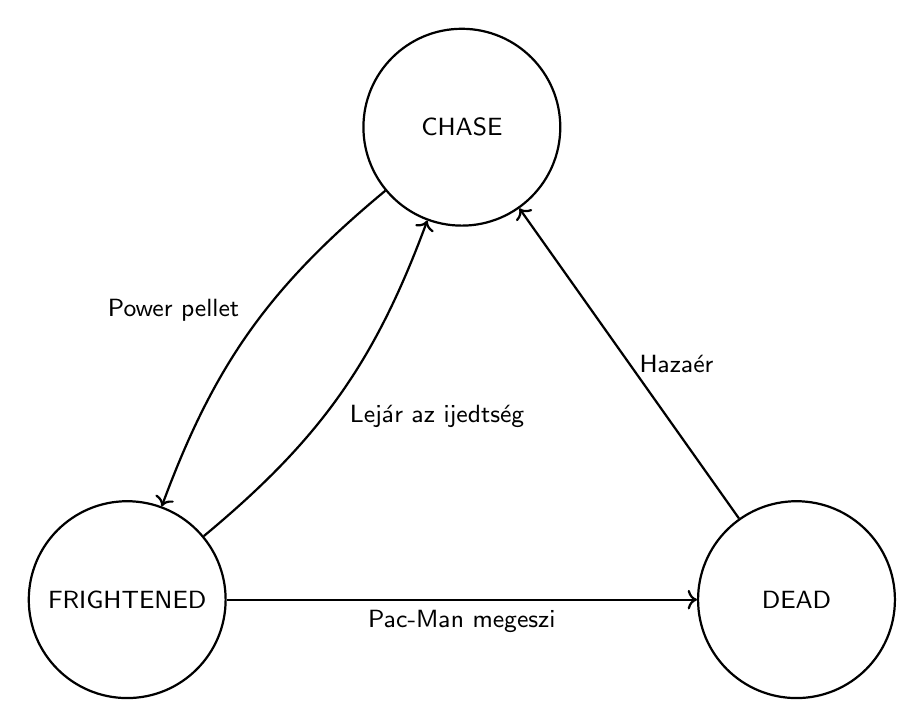
\begin{tikzpicture}[->, auto, thick,
                        every node/.style={font=\sffamily\small},
                        state/.style={draw, circle, minimum size=2.5cm, align=center}]
        
        % Az állapotok kézzel elhelyezve, a legjobb kompatibilitásért
        \node[state] (Chase) at (4.25, 0) {CHASE};
        \node[state] (Frightened) at (0, -6) {FRIGHTENED};
        \node[state] (Dead) at (8.5, -6) {DEAD};

        \path
        (Chase) edge [bend right=15] node [above left] {Power pellet} (Frightened)
        (Frightened) edge [bend right=15] node [below right] {Lejár az ijedtség} (Chase)
        (Frightened) edge node [below] {Pac-Man megeszi} (Dead)
        (Dead) edge node [right] {Hazaér} (Chase);
    \end{tikzpicture}
    } % \resizebox vége
    \caption{A szellemek viselkedésének véges állapotgépe (FSM)}
    \label{fig:ghost_fsm}
\end{figure}

\clearpage

% --- 7. Egységtesztelés ---
\section{Egységtesztelés}
A projektnek legalább \textbf{10 automatizált JUnit 5 tesztet} kell tartalmaznia. A tesztek szigorúan a logikai magra (a modellrétegre, például a \texttt{GameEngine}-re és a \texttt{Labyrinth}-ra) összpontosítanak, a Swing grafikus felület példányosítása nélkül.

Minden tesztesetnek az iparban bevett \textbf{Arrange–Act–Assert (Given–When–Then)} felépítést kell követnie:
\begin{itemize}
    \item \textbf{Arrange (Given, előkészítés):} A \texttt{GameEngine} inicializálása, egy ellenőrzött, minimális tesztpálya-mátrix betöltése és a szereplők kézi elhelyezése.
    \item \textbf{Act (When, végrehajtás):} Egy konkrét játékmechanika kiváltása (például egy mozgási parancs végrehajtása, egy \texttt{step()} futtatása vagy egy ütközés kikényszerítése). A tesztek az \texttt{update()} helyett a \texttt{step()}-et hívják, mert egy teszt játékszabályt ellenőriz, nem időzítést; és a motort rögzített seedű \texttt{Random}-mal hozzák létre, így a szellemek „véletlen” döntései minden futáskor ugyanazok.
    \item \textbf{Assert (Then, ellenőrzés):} A játékállapot várt változásainak ellenőrzése a JUnit \texttt{Assertions} segítségével (például hogy nőtt-e a pontszám, megváltoztak-e a koordináták, vagy frissült-e a szellemek állapota).
\end{itemize}

\subsection*{Kötelező tesztesetek}
A tesztkészletnek le kell fednie a kritikus játékmechanikákat, többek között az alábbiakat:
\begin{itemize}
    \item \textbf{Falnak ütközés:} \textit{Adott:} Pac-Man egy \texttt{WALL} mező mellett áll, és felé néz. \textit{Amikor:} feldolgozódik egy mozgási parancs. \textit{Akkor:} Pac-Man $(X, Y)$ koordinátái nem változhatnak.
    \item \textbf{Pötty megevése:} \textit{Adott:} Pac-Man egy \texttt{DOT} mezőre lép. \textit{Amikor:} a motor frissíti az állapotot. \textit{Akkor:} a pontszámnak nőnie kell, a mezőnek pedig \texttt{EMPTY}-re kell változnia.
    \item \textbf{Ijedt állapotba váltás:} \textit{Adott:} Pac-Man megeszik egy \texttt{POWERPELLET}-et. \textit{Amikor:} feldolgozódik az ütközés. \textit{Akkor:} minden szellemnek \texttt{CHASE} állapotból \texttt{FRIGHTENED} állapotba kell kerülnie.
    \item \textbf{Halál:} \textit{Adott:} Pac-Man és egy \texttt{CHASE} állapotú szellem ugyanazon a mezőn áll (vagy egy lépés alatt helyet cserél). \textit{Amikor:} kiértékelődnek az ütközések. \textit{Akkor:} a játékos életszámlálójának eggyel csökkennie kell, a pozícióknak pedig vissza kell állniuk a saját kezdőmezőjükre.
    \item \textbf{Game Over:} \textit{Adott:} Pac-Mannek egy élete maradt. \textit{Amikor:} összeütközik egy \texttt{CHASE} állapotú szellemmel. \textit{Akkor:} az \texttt{isGameOver()}-nek igaznak kell lennie, és a további lépések egyetlen szereplőt sem mozdíthatnak el.
\end{itemize}

\subsection*{A megvalósított tesztek}
A tesztkészlet 16 tesztből áll, 4 tesztosztályban. A tesztek a \texttt{src/test/java} mappában vannak, mindegyik a tesztelt osztállyal azonos csomagban. Minden tesztosztály egy \texttt{@BeforeEach} metódusban építi fel a közös kiinduló állapotot (fixture), így minden teszt friss állapotból indul.

\vspace{0.1cm}
\begin{tabular}{@{}p{3.6cm}p{11.2cm}@{}}
    \toprule
    \textbf{Tesztosztály} & \textbf{Mit ellenőriz} \\
    \midrule
    \texttt{GameEngineTest} (10) & falnak ütközés; pötty megevése; a blokkolt kanyar nem állítja meg az aktuális lépést; a „+” alakú mező kereszteződés; a power pellet pontot ad és megijeszti a szellemeket; egy üldöző szellemmel való találkozás egy életbe kerül, és mindenki visszaáll a kezdőmezőjére; az ijedt szellem megevése pontot ad, és az élet megmarad; a Game Over leállítja a játékot; az Ambusher 4 mezővel Pac-Man elé céloz; a \texttt{nextLevel()} növeli a szintet, és visszaállítja a megevett mezőket \\
    \texttt{GhostTest} (2) & \texttt{respawn()}: az otthonától távol lévő \texttt{DEAD} szellem \texttt{DEAD} marad; hazaérve \texttt{CHASE} lesz, és megáll \\
    \texttt{LabyrinthTest} (2) & \texttt{hasDotsLeft()}: igaz, amíg marad power pellet; hamis, ha minden elfogyott \\
    \texttt{LevelManagerTest} (2) & a hiányzó pályafájl \texttt{IOException}-t, az ismeretlen pályajel \texttt{IllegalArgumentException}-t dob (mindkettő \texttt{assertThrows}-szal, egy \texttt{@TempDir} mappában lévő fájlokon) \\
    \bottomrule
\end{tabular}
\vspace{0.1cm}

{\sloppy Együtt háromnál több osztály metódusait tesztelik, például: \texttt{GameEngine.step()}, \texttt{checkCollisions()}, \texttt{nextLevel()}, \texttt{isGameOver()}, \texttt{Labyrinth.isIntersection()}, \texttt{hasDotsLeft()}, \texttt{Ghost.frighten()}, \texttt{eaten()}, \texttt{respawn()}, \texttt{AmbusherStrategy.target()}, \texttt{MoveCommand.execute()} és \texttt{LevelManager.loadFromCSV()}.
\par}
\clearpage

% --- 8. Fájlkezelés és perzisztencia ---
\section{Fájlkezelés és perzisztencia}
\label{sec:io}
Az alkalmazás a következő adattárolási szabályokat követi, hogy az adatkezelés megbízható legyen. Minden útvonal a munkakönyvtárhoz képest relatív, ezért a játékot a projekt mappájából kell indítani.

\subsection*{1. Ranglista}
\begin{itemize}
    \item \textbf{Fájl:} \texttt{highscores.csv} a projekt mappájában (\texttt{LevelManager.HIGHSCORES\_FILE}).
    \item \textbf{Felelős:} A \texttt{LevelManager} osztály kezeli, amely az alkalmazás általános I/O segédosztálya. A pontszámot a \texttt{GamePanel} adja hozzá a játék végén; a \texttt{LeaderboardPanel} csak olvassa a fájlt.
    \item \textbf{Adatszerkezet:} Minden sornak szigorúan a \texttt{PlayerName;Score;Date} formátumot kell követnie. A dátum \texttt{yyyy-MM-dd} alakú (\texttt{LocalDate}), például \texttt{balazs;2350;2026-11-09}.
    \item \textbf{Mindig rendezett:} Az \texttt{appendHighscore(file, entry)} beolvassa az összes sort, hozzáadja az újat, pontszám szerint csökkenő sorrendbe rendezi őket, és a teljes fájlt újraírja. A lemezen lévő fájl ezért mindig megjeleníthető állapotban van, külön rendezési lépésre nincs szükség.
    \item \textbf{Olvasás:} A \texttt{loadHighscores(file)} a sorokat a legjobbal kezdve adja vissza. A hiányzó fájl nem hiba, csak üres ranglista (még senki sem fejezett be játékot). Azt a sort, amely nem \texttt{Name;Score;Date} alakú, vagy hibás a pontszáma vagy a dátuma, a sorszámával együtt elutasítja (\texttt{IllegalArgumentException}).
    \item \textbf{A játékos azonosítása:} A rendszer nem szakíthatja meg a játékost egy szövegbeviteli mezővel, hogy bekérje a nevét. Ehelyett automatikusan le kell kérnie az operációs rendszerbe éppen bejelentkezett felhasználó nevét a \texttt{System.getProperty("user.name")} hívással.
\end{itemize}

\subsection*{2. Az aktív játékállás}
Egy folyamatban lévő játék összetett állapotának (Pac-Man pontos pozíciója, minden szellem aktuális \texttt{GhostState}-je, az ijedtség-időzítőből hátralévő idő, az aktív szint és a pálya minden egyes pöttyének állapota) egyszerű szövegfájlba mentése nagyon hibalehetőséges feldolgozást igényelne.

Ezért az aktív játékállást \textbf{Java bináris szerializációval} menti a program:
\begin{itemize}
    \item \textbf{Fájlok:} mentett játékonként egy \texttt{.dat} fájl, a játékos által megadott névvel. A mentési párbeszédablak a \texttt{saves} mappában nyílik meg (\texttt{LevelManager.SAVES\_DIR}; ha hiányzik, létrejön), és a \texttt{savestate.dat} nevet ajánlja fel (\texttt{DEFAULT\_SAVE\_NAME}). A \texttt{.dat} nélkül beírt névhez a program hozzáadja a kiterjesztést, egy meglévő fájlt pedig csak megerősítés után ír felül. A \textit{Load previous game} fájlválasztója ugyanebben a mappában nyílik meg, és csak a \texttt{.dat} fájlokat mutatja, de bármelyik mentett játék kiválasztható, nem csak a legutolsó.
    \item \textbf{Megvalósítás:} A játékmag minden modellosztályának (\texttt{GameEngine}, \texttt{Labyrinth}, \texttt{GameObject}, \texttt{PacMan}, \texttt{Ghost}, a \texttt{GhostStrategy} megvalósításai és az enumok) meg kell valósítania a \texttt{java.io.Serializable} interfészt. A \texttt{LevelData} csak a \texttt{LevelManager}-től a \texttt{GameEngine}-ig utazik, és nem kerül mentésre, ezért neki nem kell. A motor \texttt{java.util.Random} példánya maga is szerializálható, az egyszerű számlálók (\texttt{tickInStep}, \texttt{stepCount}), a szint labirintus-pillanatképe (\texttt{originalMap}) és minden szereplő kezdő- és előző mezője pedig automatikusan mentődik.
    \item \textbf{Ami nem mentődik:} A \texttt{PacMan.currentCommand} \texttt{transient}. A \texttt{MoveCommand} nem \texttt{Serializable}, és a pufferelt billentyűlenyomás bemenet, nem játékállapot, így a betöltött játék függőben lévő kanyar nélkül indul.
    \item \textbf{Végrehajtás:} A \texttt{GameEngine} \texttt{saveGameState(file)} metódusa a teljes motorpéldányt bináris fájlba írja egy \texttt{ObjectOutputStream} segítségével. A statikus \texttt{loadGameState(file)} egy \texttt{ObjectInputStream}-mel olvassa vissza, és új motorként adja vissza, kézi adatleképezés nélkül, pontosan visszaállítva az állapotot. Ha a fájl más objektumot tartalmaz, a program \texttt{IOException}-ként jelzi („Not a Pac-Man save file”), ugyanúgy, mint minden más olvashatatlan fájlt, és a menü összeomlás helyett hibaüzenetet mutat.
    \item \textbf{Korlát:} A modellosztályok nem deklarálnak \texttt{serialVersionUID}-t, ezért a Java az osztály szerkezetéből számol egyet. Egy modellosztály megváltozása után a régi változattal készült mentések már nem tölthetők be (\texttt{InvalidClassException}, amely betöltési hibaként jelenik meg).
\end{itemize}

\subsection*{3. Pályák}
\label{sec:custom_maps}
\begin{itemize}
    \item \textbf{Formátum:} A beépített pályák és a \texttt{MapEditor}-ral készült pályák is olyan szövegfájlok, amelyek magát a labirintust ábrázolják: soronként a labirintus egy sora, mezőnként egy karakter. A \texttt{LevelManager} soronként olvassa be őket a \texttt{loadFromCSV}-vel, és a \texttt{saveToCSV}-vel írja ki. Minden pálya a \texttt{maps} mappában van (\texttt{LevelManager.MAPS\_DIR}). A beépített pálya a \texttt{maps/level1.txt}; a \textit{Start new game} ezt ajánlja fel először, de bármelyik pályafájl kiválasztható.
    \item \textbf{Jelek:}

    \vspace{0.2cm}
    \begin{tabular}{@{}cll@{}}
        \toprule
        \textbf{Karakter} & \textbf{Jelentés} & \textbf{Tárolás} \\
        \midrule
        \texttt{\#} & Fal & \texttt{CellType.WALL} \\
        \texttt{.} & Pötty & \texttt{CellType.DOT} \\
        \texttt{o} & Power pellet & \texttt{CellType.POWERPELLET} \\
        \texttt{\_} & Üres padló & \texttt{CellType.EMPTY} \\
        \texttt{P} & Pac-Man kezdőmezője (pontosan egy) & \texttt{PacMan} egy \texttt{EMPTY} mezőn \\
        \texttt{T} & Egy \texttt{TRACKER} szellem kezdőmezője & \texttt{Ghost} egy \texttt{EMPTY} mezőn \\
        \texttt{A} & Egy \texttt{AMBUSHER} szellem kezdőmezője & \texttt{Ghost} egy \texttt{EMPTY} mezőn \\
        \texttt{W} & Egy \texttt{WANDERER} szellem kezdőmezője & \texttt{Ghost} egy \texttt{EMPTY} mezőn \\
        \texttt{C} & Egy \texttt{CHAOTIC} szellem kezdőmezője & \texttt{Ghost} egy \texttt{EMPTY} mezőn \\
        \bottomrule
    \end{tabular}
    \vspace{0.2cm}

    \item \textbf{Miért karakterek, és miért nem \texttt{CellType} nevek:} Egy \texttt{CellType} mátrix csak mezőket tud leírni, így nem tudja rögzíteni, hol kezd Pac-Man és a szellemek. A karakteres rajz mindkettőt tárolja, olvasható marad, és kézzel is szerkeszthető. A szellemek kezdőmezői egyben a szellemházat is kijelölik, ahová a \texttt{DEAD} szellemek visszatérnek.
    \item \textbf{Ellenőrzés:} Minden sornak azonos hosszúnak kell lennie, pontosan egy \texttt{P} kell, és minden más karaktert (a szóközt is) a program a sorával és oszlopával együtt elutasít. Az üres sorokat és a sorvégi szóközöket figyelmen kívül hagyja, ezért jelöli az üres padlót \texttt{\_}, és nem szóköz. A szerkesztőben készült pályák ezen felül mindig $19 \times 21$ méretűek, rögzített szellemházzal és legalább egy pöttyel; a kézzel írt pályafájlok bármekkorák lehetnek.
    \item \textbf{Példa} (egy kis labirintus Pac-Mannel, egy power pellettel és két szellemmel):

    \vspace{0.1cm}
\begin{verbatim}
#########
#P..o...#
#.##_##.#
#..T_A..#
#########
\end{verbatim}
\end{itemize}

\clearpage

% --- 9. Felhasználói kézikönyv ---
\section{Felhasználói kézikönyv}
\label{sec:manual}

\subsection*{A program indítása}
A játékhoz Java 17 vagy újabb szükséges. Fordítsa le az \texttt{mvn compile} paranccsal, majd indítsa a projekt mappájából (abból a mappából, amelyben a \texttt{maps} található):

\vspace{0.1cm}
\texttt{java -cp target/classes hu.bme.pacman.system.Main}
\vspace{0.1cm}

Ha fejlesztőkörnyezetből (IDE) indítja, a munkakönyvtárnak ott is a projekt mappájának kell lennie. A játék minden fájlját (pályák, mentések, ranglista) ehhez képest keresi.

\subsection*{Főmenü}
\begin{itemize}
    \item \textbf{Start new game:} fájlválasztó nyílik a \texttt{maps} mappában, a beépített \texttt{level1.txt} kijelölésével. Válasszon pályát, és nyomja meg az \textit{Open} gombot; a játék 0 ponttal, 3 élettel, az 1. szinten indul. A \textit{Cancel} visszavisz a menübe.
    \item \textbf{Load previous game:} fájlválasztó nyílik a \texttt{saves} mappában. Válasszon egy mentett játékot (\texttt{.dat}); pontosan ott folytatódik, ahol mentette.
    \item \textbf{Leaderboard:} a befejezett játékok listája.
    \item \textbf{Create map:} megnyitja a pályaszerkesztőt.
\end{itemize}

\subsection*{Játék}
\begin{itemize}
    \item \textbf{Irányítás:} \texttt{W} fel, \texttt{A} balra, \texttt{S} le, \texttt{D} jobbra. Pac-Man addig halad a saját irányába, amíg falhoz nem ér, ott megáll. A kanyar előre is lenyomható: Pac-Man megjegyzi az utolsó billentyűt, és az első olyan mezőn fordul, ahol arra szabad az út, így a kanyarok megállás nélkül bevehetők.
    \item \textbf{Cél:} a labirintus minden pöttyének és power pelletjének megevése. Ezután ugyanazon a pályán indul a következő szint, újra minden pöttyel; a pontszám és a megmaradt életek megmaradnak.
    \item \textbf{Állapotsor} (a képernyő tetején): pontszám, megmaradt életek, aktuális szint, \texttt{GAME OVER}, ha már nincs élet, és a \textit{SAVE \& QUIT} gomb.
    \item \textbf{Pontok:}

    \vspace{0.1cm}
    \begin{tabular}{@{}ll@{}}
        \toprule
        \textbf{Amit Pac-Man megeszik} & \textbf{Pont} \\
        \midrule
        Pötty (kis fehér pont) & 10 \\
        Power pellet (nagy fehér pont) & 50 \\
        Szellemek egy power pellet után & 200, 400, 800, majd minden további szellemért 1600 \\
        \bottomrule
    \end{tabular}
    \vspace{0.1cm}

    \item \textbf{Szellemek:} a labirintus közepén lévő szellemházból indulnak.
    \begin{itemize}
        \item Piros (Tracker): egyenesen Pac-Man felé tart.
        \item Rózsaszín (Ambusher): 4 mezővel Pac-Man elé céloz, hogy elvágja az útját.
        \item Narancssárga (Wanderer): üldözi Pac-Mant, de visszafordul haza, ha 8 mezőnél közelebb kerül hozzá.
        \item Cián (Chaotic): 15 másodpercenként átvált a másik három viselkedés egyikére.
    \end{itemize}
    \item \textbf{Power pellet:} minden szellem fehér lesz, megfordul, és fele sebességgel kóborol; ilyenkor Pac-Man megeheti őket. A hatás az 1--3. szinten 6, a 4--6. szinten 4, a 7--10. szinten 2 másodpercig tart, a 11. szinttől 1 másodpercig. A megevett szellem kis szürke ponttá (a szemévé) válik: ártalmatlan, visszasiet a szellemházba, és ott visszaváltozik.
    \item \textbf{Életvesztés:} egy színes szellem érintése egy életbe kerül. Pac-Man és az összes szellem visszakerül a kezdőmezőjére; az addig megevett pöttyök nem jönnek vissza.
    \item \textbf{Game over:} amikor az utolsó élet is elfogy, megjelenik a \texttt{GAME OVER} felirat, és a pontszám automatikusan bekerül a ranglistába, a számítógépre bejelentkezett felhasználó nevével. A játék nem kér nevet. Ezután a \textit{SAVE \& QUIT} (vagy az \texttt{F5}) mentés nélkül visszalép a főmenübe.
\end{itemize}

\subsection*{Játékállás mentése és betöltése}
\begin{itemize}
    \item A \texttt{GAME OVER} előtt bármikor megnyomhatja a \textit{SAVE \& QUIT} gombot vagy az \texttt{F5} billentyűt. A játék szünetel, és mentési párbeszédablak nyílik a \texttt{saves} mappában, a \texttt{savestate.dat} név felajánlásával. Bármilyen név beírható; ha hiányzik, a program hozzáadja a \texttt{.dat} kiterjesztést, meglévő fájl felülírása előtt pedig megerősítést kér. Mentés után a játék visszalép a főmenübe.
    \item Ha a párbeszédablakot bezárja, vagy a mentés nem sikerül, a játék egyszerűen folytatódik.
    \item A \texttt{saves} mappában tetszőleges számú játék tárolható; a \textit{Load previous game} bármelyiket meg tudja nyitni. A közvetlenül mentés előtt lenyomott kanyar nem marad meg: betöltés után nyomja meg újra az irányt.
    \item A program egy régebbi változatával készült mentés a program megváltozása után esetleg nem tölthető be; ilyenkor hibaüzenet jelenik meg, és a menü nyitva marad.
\end{itemize}

\subsection*{Ranglista}
A program minden befejezett játékot felsorol a helyezésével, a játékos nevével, a pontszámmal és a dátummal, a legjobb pontszámtól a leggyengébbig. A \textit{Back to menu} visszavisz a főmenübe.

\subsection*{Pályaszerkesztő}
\begin{itemize}
    \item \textbf{A rács:} a szerkesztő egy üres, fekete, $19 \times 21$ mezős pályával nyílik meg, amely akkora, mint a beépített pálya; más méret nem lehetséges. A középen lévő szellemház (sötétszürke mezők a négy szellemmel) rögzített: nem lehet ráírni, és szellemet máshová nem lehet lerakni.
    \item \textbf{Eszközök} (jobb oldalt): \textit{WALL} (kék fal), \textit{DOT} (kis fehér pötty), \textit{POWER PELLET} (nagy fehér pont) és \textit{PAC-MAN START} (Pac-Man kezdőmezője). Egy eszközt a gombjára kattintva lehet kiválasztani.
    \item \textbf{Rajzolás:} a \textbf{bal} egérgombbal egy mezőre kattintva a kiválasztott eszköz rákerül, a gombot lenyomva tartva és az egeret húzva pedig minden érintett mezőre.
    \item \textbf{Törlés:} a \textbf{jobb} egérgombbal egy mezőre kattintva (vagy azzal húzva) a mező újra üres padló lesz.
    \item \textbf{Pac-Man kezdőmezője:} legfeljebb egy lehet. Másik mezőre lerakva oda kerül át; ha a mezőjére rajzol vagy törli, eltűnik.
    \item \textbf{Keret:} a rácson kívüli mezők falnak számítanak, így falkeret nélkül sem hagyhatja el semmi a pályát; keretet rajzolni nem kötelező.
    \item \textbf{SAVE MAP:} a pálya csak akkor menthető, ha Pac-Man kezdőmezője le van rakva, és van legalább egy pötty; ha nem, egy üzenet megmondja, mi hiányzik. A mentési párbeszédablak a \texttt{maps} mappában nyílik meg; írjon be egy nevet (ha hiányzik, a program hozzáadja a \texttt{.txt}-t). A \texttt{level1.txt} nem írható felül, egy másik pálya felülírása előtt pedig megerősítést kér. Mentés után a szerkesztő nyitva marad.
    \item \textbf{BACK:} visszalép a főmenübe. Ha a pályán még nem mentett változás van, előbb rákérdez.
    \item \textbf{Játék az új pályán:} a \textit{Start new game} után válassza ki a fájlválasztóban.
    \item \textbf{Tippek:} a szerkesztő nem ellenőrzi, hogy Pac-Man minden pöttyöt elér-e. Az elérhetetlen pöttyöt tartalmazó szint sosem fejezhető be, ezért minden pöttyhöz hagyjon utat. A szellemház nyílásai körüli mezőket is hagyja szabadon, különben a szellemek nem tudnak kijönni.
\end{itemize}

\subsection*{A játék fájljai}
\begin{tabular}{@{}ll@{}}
    \toprule
    \textbf{Fájl vagy mappa} & \textbf{Tartalom} \\
    \midrule
    \texttt{maps/} & Pályák (\texttt{.txt}): a beépített \texttt{level1.txt} és a szerkesztőben rajzolt pályák \\
    \texttt{saves/} & Mentett játékok (\texttt{.dat}) \\
    \texttt{highscores.csv} & A ranglista, soronként egy befejezett játék \\
    \bottomrule
\end{tabular}

\subsection*{Ismert korlátok}
\begin{itemize}
    \item Az ablak bezárása azonnal kilép a programból, és nem kérdez rá a mentetlen játékra vagy pályára.
\end{itemize}

\end{document}
